\documentclass{article}

\usepackage[T1]{fontenc}
\usepackage[utf8]{inputenc}
\usepackage[french,english]{babel}
\usepackage{graphicx}
\usepackage{hyperref}
\usepackage{listings}
\usepackage{amsmath}
\usepackage{minted}

\title{%
  Rapport de Projet : Simulateur de Réseaux et Trafic Cycliste%
}

\author{Lucas Goddet - Khanh Huyen Vu}
\date{28 Février 2026}

\begin{document}
\maketitle

\section{Introduction}

\paragraph{Objectif du projet.}
Notre projet a pour but la conception d'un simulateur de réseaux dans lequel nous simulerons le trafic de cyclistes. Originalement conçu pour simuler des envois de paquets entre routeurs, nous avons fait évoluer le projet en une version où nous simulons un parc de vélos. Le simulateur permet d'observer comment un algorithme de routage s'adapte en temps réel à la congestion du trafic qui sera générée par l'afflux de cyclistes dans les différentes rues empruntées.

\paragraph{Métrique de succès.}
Pour juger de la réussite de ce projet, nous avons défini que la réussite de ce projet revenait à pouvoir valider ces différents points :
\begin{itemize}
    \item \textbf{Convergence algorithmique :} Le réseau doit être capable de trouver des chemins optimaux sans créer de boucles de routage (éviter le problème de \textit{Count-to-Infinity} en utilisant la méthode \textit{Split Horizon}).
    \item \textbf{Réactivité au trafic :} Si un lien (une rue) voit son coût augmenter à cause d'une trop forte affluence de cyclistes, le réseau doit rediriger les cyclistes suivants vers des chemins alternatifs viables de manière autonome.
    \item \textbf{Scalabilité visuelle et technique :} Le simulateur doit être capable de gérer et d'afficher clairement un graphe de plusieurs dizaines de nœuds et utilisateurs, sans crash et sans perte de lisibilité des données.
    \item \textbf{Exploitation de données :} La capacité à générer un réseau non plus manuellement, mais en lisant un jeu de données réel (fichiers de l'Open Data).
\end{itemize}

\section{Implémentation}

\paragraph{Réalisation et logiciel codé.}
Le simulateur est développé sous la forme d'un moteur temporel utilisant un système de \textit{ticks} (actualisation étape par étape du simulateur). À chaque tick, les nœuds s'échangent des messages pour mettre à jour leurs tables de routage, puis les cyclistes interrogent ces tables pour avancer d'une station à l'autre. Le coût des liens est recalculé dynamiquement à chaque itération en fonction du nombre de cyclistes présents sur l'arête.

\paragraph{Structure en modules.}
L'architecture logicielle respecte une séparation des responsabilités à l'aide de plusieurs modules :
\begin{itemize}
    \item {\tt network.py} : Gère la topologie, sauvegarde l'historique et calcule la congestion.
    \item {\tt router.py} et algorithmes : Représentent les stations et implémentent l'algorithme \textit{Distance Vector}.
    \item {\tt user.py} : Modélise les cyclistes qui se déplacent sur le graphe.
    \item {\tt visualizer.py} : L'interface graphique interactive.
\end{itemize}

\paragraph{Représentation des données.}
Le réseau est conceptuellement un graphe pondéré. Les données à chaque tick sont sérialisées sous forme de dictionnaires primitifs : une topologie associant des paires de routeurs à un coût, des tables de routage allégées, et une liste d'états pour les cyclistes.

\paragraph{Technologies utilisées.}
Le projet utilise le langage {\tt Python 3}. Pour la visualisation et la modélisation du graphe, le code utilise les bibliothèques {\tt NetworkX} et {\tt Matplotlib}. 
La Figure~\ref{fig:visualizer} montre le rendu de notre interface.
\begin{figure}[H]
\label{fig:visualizer}
\hrulefill
\begin{center}
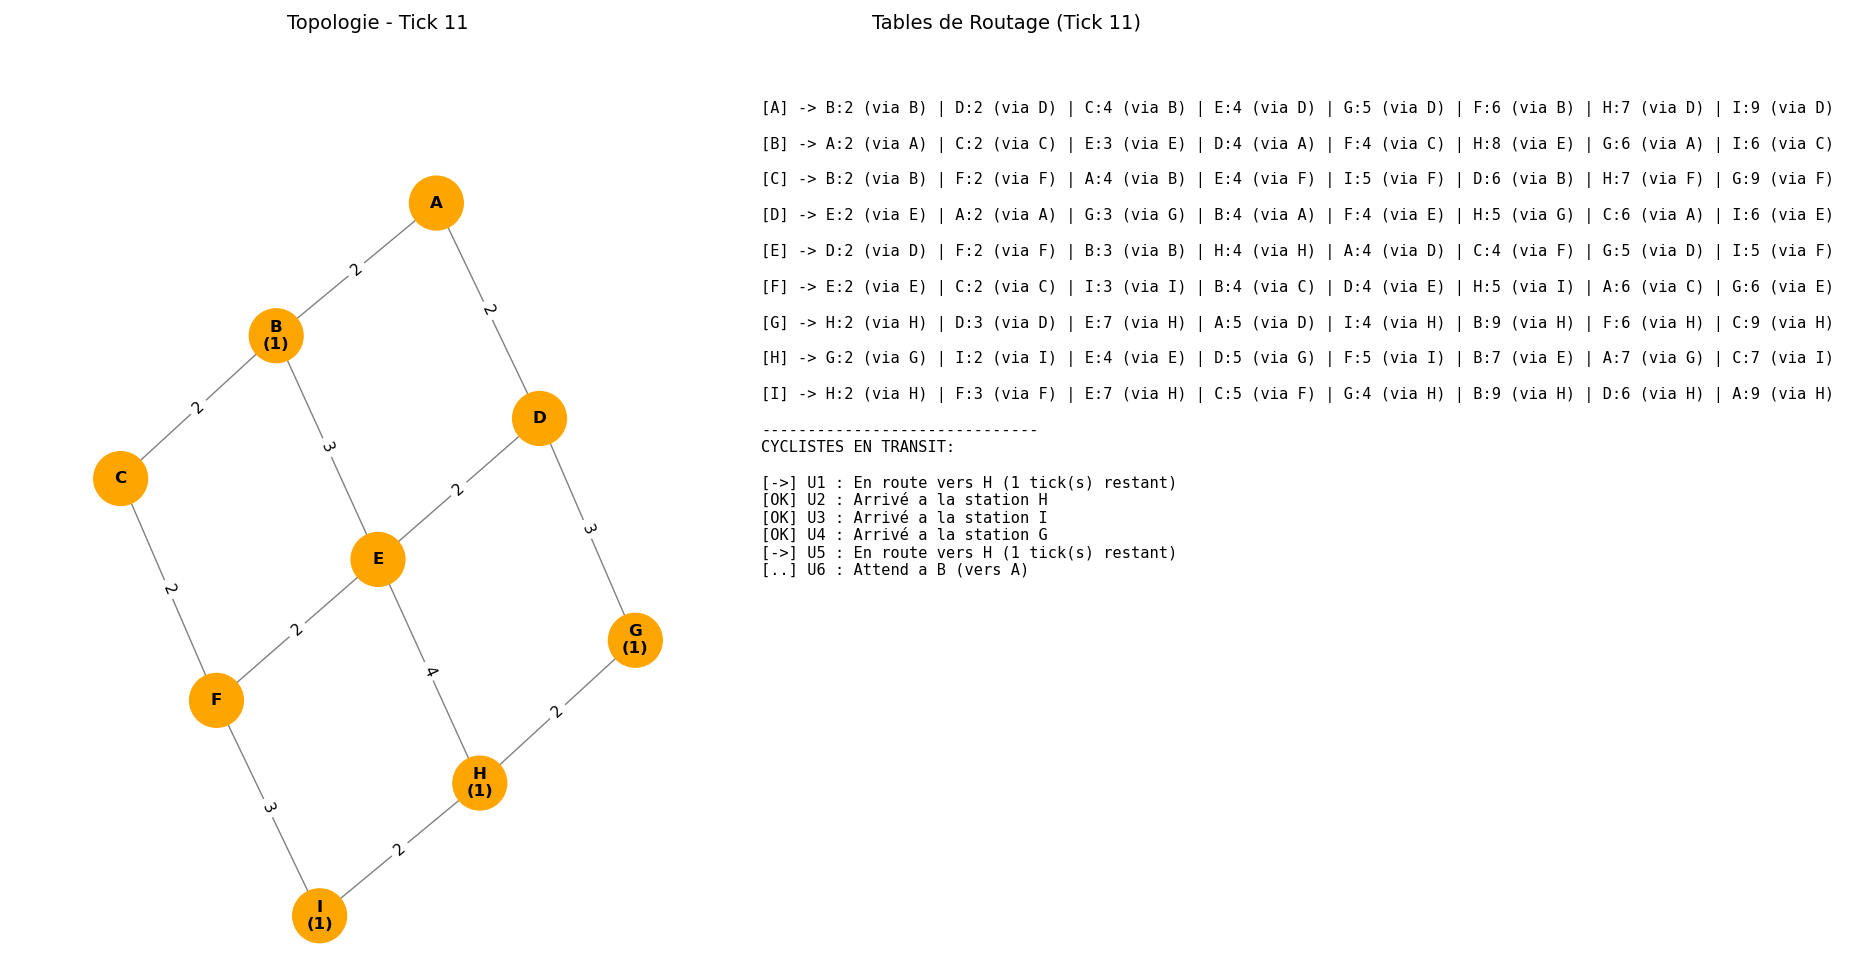
\includegraphics[height=80px,width=230px]{visualizer.png}
\end{center}
\caption{Interface du visualiseur interactif : topologie à gauche, tables de routage et état des cyclistes à droite.}
\hrulefill
\end{figure}

\paragraph{Extrait de code : Moteur temporel.}
L'extrait ci-dessous illustre la mise à jour dynamique du trafic à chaque itération.
\begin{figure}[H]
\label{code:tick}
\hrulefill
\inputminted[breaklines, fontsize=\small, firstline=72, lastline=86 ]{python}{network.py}
\hrulefill
\end{figure}

\paragraph{Extrait de l'algorithme de routage.} Le code de la Figure~\ref{code:distance-vector} montre comment chaque station traite les messages reçus de ses voisins pour mettre à jour sa table de routage si un chemin plus rapide est trouvé ou si le coût d'une rue change.
\begin{figure}[H]
\label{code:distance-vector}
\hrulefill
\inputminted[breaklines, fontsize=\small, firstline=29, lastline=48]{python}{distance_vector.py}
\hrulefill
\end{figure}

\section{Jalons}

\paragraph{Tâches déjà terminées.}
Le socle de la simulation est opérationnel :
\begin{itemize}
    \item Implémentation de l'algorithme \textit{Distance Vector}.
    \item Moteur visuel fonctionnel avec historique permettant de naviguer dans les différents ticks de l'algorithme.
    \item Création des cyclistes capables de lire les tables et de se déplacer.
    \item Module de congestion dynamique.
\end{itemize}

\paragraph{Tâches à réaliser.}
Les tâches qu'il nous reste à réaliser pour finaliser le projet sont :
\begin{enumerate}
    \item \textbf{Parseur :} Développer un script pour extraire une sous-partie des données de l'Open Data.
    \item \textbf{Inclusion d'Open Data :} Construire automatiquement le graphe à partir de ces fichiers externes.
    \item \textbf{Gestion des inventaires :} Ajouter une capacité maximale de vélos et de places à chaque station.
    \item \textbf{Cycle journalier :} Implémenter une notion d'heure pour simuler les "heures de pointe".
\end{enumerate}

\paragraph{Organisation temporelle.}
Le schéma ci-dessous illustre notre diagramme de Gantt pour les semaines à venir.

\begin{figure}[htbp]
\label{fig:gantt}
\hrulefill
\begin{center}
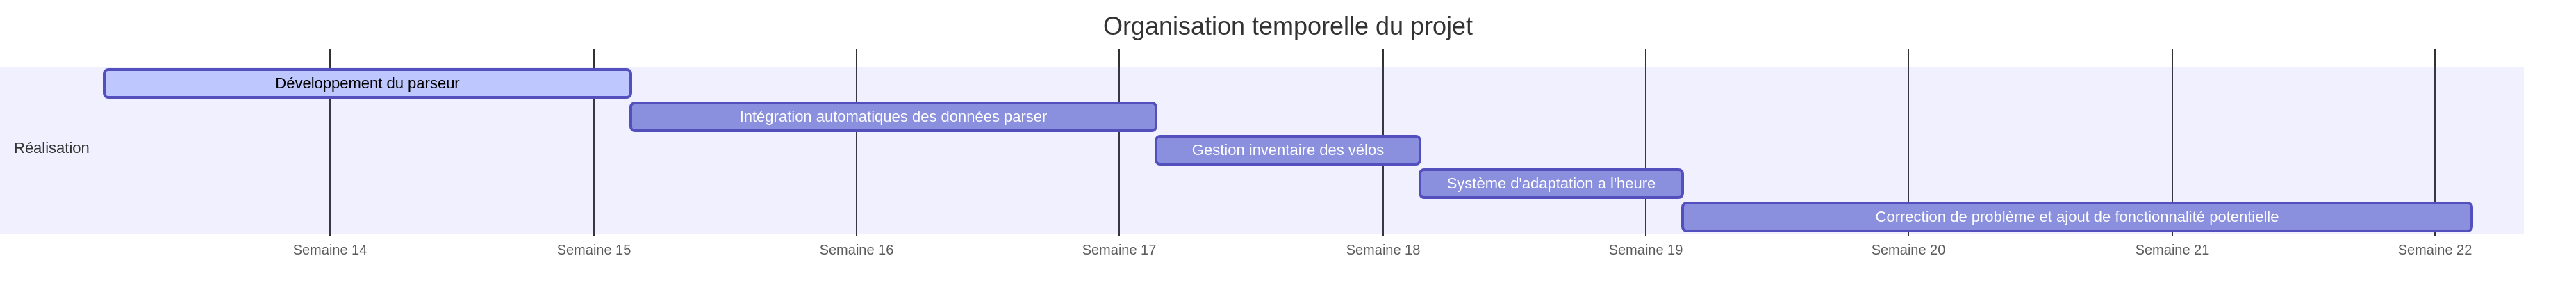
\includegraphics[width=\linewidth]{gantt.png}
\end{center}
\caption{Schéma de l'organisation temporelle des tâches.}
\hrulefill
\end{figure}

\end{document}
